% Compile with XeLaTeX.
% Theme: gemini + Stanford colors (Stanford-LaTeX-Poster-Template).

\documentclass[final]{beamer}

% ====================
% Packages
% ====================
\usepackage[T1]{fontenc}
\usepackage{lmodern}
\usepackage[size=custom,width=120,height=72,scale=1.0]{beamerposter}
\usetheme{gemini}
\usecolortheme{stanford}
\usepackage{graphicx}
\usepackage{booktabs}
\usepackage{colortbl}
\usepackage{tikz}
\usepackage{pgfplots}
\pgfplotsset{compat=1.17}
\usetikzlibrary{arrows.meta,positioning,shapes.geometric,calc,backgrounds}

% ====================
% Role colors (consistent everywhere)
% ====================
\colorlet{adjcol}{darkorange}      % adjective  (describes)
\colorlet{nouncol}{skyblue}        % subject noun (the thing)
\colorlet{verbcol}{treegreen}      % verb       (the action)
\colorlet{objcol}{darkpurple}      % object     (acted upon)
\colorlet{poscol}{treegreen}
\colorlet{negcol}{cardinalred}
\colorlet{hi}{darkbeige}

\newcommand{\wordbox}[2]{%
  \tikz[baseline=(w.base)]{\node[rounded corners=4pt, draw=#1, line width=1.4pt,
    fill=#1!12, text=#1!60!black, inner sep=7pt, font=\bfseries] (w) {#2};}}

% ====================
% Lengths (3 columns)
% ====================
\newlength{\sepwidth}
\newlength{\colwidth}
\setlength{\sepwidth}{0.025\paperwidth}
\setlength{\colwidth}{0.3\paperwidth}
\newcommand{\separatorcolumn}{\begin{column}{\sepwidth}\end{column}}

\title{Can a Quantum Circuit Read a Sentence?}
\author{Feolu Kolawole \enspace$\cdot$\enspace Nick Rui \\[0.3ex]
  {\normalsize Turning ``the clever program runs'' into a trained 2-qubit circuit --- worked end to end}}
\institute[shortinst]{Physics 14N \enspace$\cdot$\enspace Stanford University}
\footercontent{\hfill From Syntax to Circuits: a toy QNLP sentiment classifier \hfill
  \href{mailto:flukol@stanford.edu}{flukol@stanford.edu}}

\begin{document}

\addtobeamertemplate{headline}{}
{
    \begin{tikzpicture}[remember picture,overlay]
      \node [anchor=north east, inner sep=3cm] at ([xshift=0.0cm,yshift=2.5cm]current page.north east)
      {
\includegraphics[height=7.0cm]{stanford_logos/Block_S_2_color.png}};
    \end{tikzpicture}
}

\begin{frame}[t]
\begin{columns}[t]
\separatorcolumn

% =====================================================================
% COLUMN 1 --- the idea, grammar (+weights), the qubit
% =====================================================================
\begin{column}{\colwidth}

  \begin{block}{The goal}
    Read a short sentence and decide \textbf{\color{poscol}positive} or
    \textbf{\color{negcol}negative} (its \textbf{sentiment}) --- but do it the way
    \textbf{Quantum NLP} does: turn the words into a \textbf{quantum circuit} and let a
    measurement give the answer.
    \smallskip
    \begin{center}\normalsize
      \textbf{\color{poscol}positive$=$good$=$YES$=1$} \quad$\mid$\quad
      \textbf{\color{negcol}negative$=$bad$=$NO$=0$}
    \end{center}
  \end{block}

  \begin{alertblock}{The whole pipeline in one line}
    \begin{center}\large
      \textbf{words $\to$ dials} \;$\cdot$\; \textbf{grammar $\to$ wiring \& weights}
      \;$\cdot$\; \textbf{circuit $\to$ measure $\to$ answer}
    \end{center}
    Each word owns one \textbf{learned number}. Grammar decides how those numbers are
    combined. A quantum measurement turns the result into a probability of
    ``\textbf{\color{poscol}positive}.''
  \end{alertblock}

  \begin{block}{Step 1 --- Grammar gives each word a role \emph{and} a weight}
    Our sentences follow one shape; each word plays a colored \textbf{role}:
    \begin{center}\large
      \wordbox{adjcol}{clever}\;\wordbox{nouncol}{program}\;\wordbox{verbcol}{runs}
      \;\wordbox{objcol}{(the puzzle)}
    \end{center}
    \begin{center}\footnotesize
      {\color{adjcol!60!black}\textbf{adjective}}\quad
      {\color{nouncol!60!black}\textbf{subject}}\quad
      {\color{verbcol!60!black}\textbf{verb}}\quad
      {\color{objcol!60!black}\textbf{object}}
    \end{center}

    Grammar says \emph{who connects to whom} --- and \textbf{how much each role counts}.
    The verb and adjective carry sentiment; the bare nouns barely matter:

    \begin{center}
      \begin{tabular}{lc}
        \toprule
        \textbf{role} & \textbf{weight} \\
        \midrule
        {\color{verbcol!60!black}verb} (the action)        & \textbf{1.40} \\
        {\color{adjcol!60!black}adjective} (describes)      & \textbf{1.25} \\
        object-adjective                                    & 0.90 \\
        {\color{nouncol!60!black}subject} (the thing)       & 0.45 \\
        {\color{objcol!60!black}object} (acted on)          & 0.35 \\
        \bottomrule
      \end{tabular}
    \end{center}
    \footnotesize (Object roles only kick in for longer sentences with an object ---
    ours, ``the clever program runs,'' uses just the top, subject, and verb.)
  \end{block}

  \begin{block}{Step 2 --- A qubit is a dial, and measuring squares it}
    A \textbf{bit} is a switch: \textbf{0} or \textbf{1}. A \textbf{qubit} is a
    \textbf{dial} that can point anywhere between \textbf{\color{negcol}NO} (0) and
    \textbf{\color{poscol}YES} (1). \textbf{What's quantum:} until you look it holds a
    real \textbf{blend} of both at once.

    \begin{itemize}
      \item A dial tilted by angle $\theta$ carries \textbf{amplitude}
            $\cos(\theta/2)$ on NO and $\sin(\theta/2)$ on YES.
      \item \textbf{Measuring is random; the rule is: probability $=$ amplitude$^2$.}
            A dial leaning far to YES has a big YES-amplitude $\Rightarrow$ reads YES
            almost every time. Straight up $=$ 50/50.
    \end{itemize}
    We use \textbf{two} dials: a \textbf{\color{nouncol}subject dial} and a
    \textbf{\color{verbcol}sentence dial} (it ends up holding the answer). For both
    dials at once, \textbf{multiply} their amplitudes for each reading.
  \end{block}

\end{column}

\separatorcolumn

% =====================================================================
% COLUMN 2 --- words to angles, the circuit, the CX gate
% =====================================================================
\begin{column}{\colwidth}

  \begin{block}{Step 3 --- Turning words into rotation angles}
    Each word's learned number is how far it \textbf{rotates} a dial. Grammar adds the
    right words onto each wire. For \wordbox{poscol}{the clever program runs}, the
    \emph{trained} dials are
    \;{\color{adjcol!60!black}\textbf{clever}}$=0.098$,\;
    {\color{nouncol!60!black}\textbf{program}}$=0.043$,\;
    {\color{verbcol!60!black}\textbf{runs}}$=0.489$:

    \medskip
    \begin{center}\large
    \begin{tabular}{r l}
      {\color{nouncol!60!black}\textbf{subject angle}}  & $=$ clever $+$ program $= 0.098+0.043 = \mathbf{0.141}$\\[4pt]
      {\color{verbcol!60!black}\textbf{sentence angle}} & $=$ runs $= \mathbf{0.489}$\\[4pt]
      \textbf{decision angle} & $=\ \underbrace{\pi/2}_{\text{start straight up}}+\ \underbrace{\text{score}}_{\text{weighted words}}$\\[10pt]
      \multicolumn{2}{r}{$\text{score}=\underbrace{0.068}_{\text{bias}}+1.25(0.098)+0.45(0.043)+1.40(0.489)=0.894$}\\[6pt]
      \multicolumn{2}{r}{decision angle $=\pi/2+0.894=\mathbf{2.465}$}
    \end{tabular}
    \end{center}
    \smallskip
    The decision dial starts \textbf{straight up} (the 50/50 line) so the weighted words
    can push it either way --- and the \textbf{verb} pushes hardest (weight 1.40).

    \medskip
    \begin{center}
    \begin{tikzpicture}[font=\sffamily,
        gate/.style={draw, rounded corners=2pt, line width=1pt, minimum width=2.0cm, minimum height=1.05cm, align=center, font=\small},
        wire/.style={line width=1.3pt}]
      \draw[wire, nouncol] (3,1.4) -- (16.2,1.4);
      \draw[wire, verbcol] (3,-1.6) -- (16.2,-1.6);
      \node[nouncol!60!black, font=\small\bfseries, anchor=east] at (2.8,1.4) {subject};
      \node[verbcol!60!black, font=\small\bfseries, anchor=east] at (2.8,-1.6) {sentence};
      \node[gate, fill=nouncol!15] at (5.2,1.4)  {tilt\\0.141};
      \node[gate, fill=verbcol!15] at (5.2,-1.6) {tilt\\0.489};
      \fill[cardinalred] (8.6,1.4) circle (6pt);
      \draw[cardinalred, line width=1.6pt] (8.6,1.4) -- (8.6,-1.6);
      \draw[cardinalred, line width=1.6pt] (8.6,-1.6) circle (10pt);
      \draw[cardinalred, line width=1.6pt] (8.28,-1.6) -- (8.92,-1.6);
      \node[cardinalred, font=\small\bfseries, align=center] at (8.6,2.5) {CX (link)};
      \node[gate, fill=coolgray!22] at (11.7,-1.6) {tilt\\2.465};
      \node[draw, line width=1.3pt, rounded corners=3pt, minimum width=1.9cm, minimum height=1.3cm] (meter) at (14.7,-1.6) {};
      \draw[line width=1pt] ([xshift=-0.55cm,yshift=-0.3cm]meter.center) arc (180:0:0.55);
      \draw[-{Latex[length=3mm]}, line width=1.1pt] ([yshift=-0.3cm]meter.center) -- ++(38:0.65);
      \node[font=\small\bfseries, below=1mm of meter] {measure};
    \end{tikzpicture}
    \end{center}
    \footnotesize ``\textbf{tilt $\theta$}'' just means \emph{rotate that dial by angle
    $\theta$} (physicists call it an \emph{Ry} gate). The sentence dial is tilted
    \textbf{twice}: first by its own word ($0.489$), then by the whole weighted verdict
    ($2.465$).
  \end{block}

  \begin{alertblock}{Step 4 --- The CX gate: grammar's glue (and the quantum part)}
    Grammar says the \textbf{\color{nouncol}subject} and the \textbf{\color{verbcol}action}
    are \textbf{one} sentence, so we link their dials with a \textbf{CX gate}. Its rule
    (\textbf{C}\,=\,control/check, \textbf{X}\,=\,flip):
    \begin{center}\large
      \textbf{If the \color{nouncol}subject\color{black}\ reads
      \color{poscol}YES\color{black}, flip the \color{verbcol}sentence\color{black}\ dial;
      if \color{negcol}NO\color{black}, leave it.}
    \end{center}

    \heading{Literally, on the four readings}
    The two dials together have four readings (left digit $=$ subject, right $=$ sentence).
    CX just \textbf{swaps the two where the subject reads 1} ($10\leftrightarrow11$):
    \begin{center}\large
      \begin{tabular}{lcccc}
        \toprule
         & \textbf{00} & \textbf{01} & \cellcolor{hi!40}\textbf{10} & \cellcolor{hi!40}\textbf{11}\\
        \midrule
        before & 0.968 & 0.241 & \cellcolor{hi!40}0.068 & \cellcolor{hi!40}0.017\\
        after  & 0.968 & 0.241 & \cellcolor{hi!40}0.017 & \cellcolor{hi!40}0.068\\
        \bottomrule
      \end{tabular}
    \end{center}

    Because each dial is still a \textbf{blend}, this welds their answers together ---
    like \textbf{two coins glued}: you can't flip one without the other. They are now
    \textbf{entangled}, and no separate spinning can fake that link.
  \end{alertblock}

\end{column}

\separatorcolumn

% =====================================================================
% COLUMN 3 --- the literal end-to-end run + results
% =====================================================================
\begin{column}{\colwidth}

  \begin{block}{Watch one sentence compute, slot by slot}
    The two dials together have four possible readings: \textbf{00, 01, 10, 11}
    (\textbf{left digit $=$ \color{nouncol}subject dial}, \textbf{right digit $=$
    \color{verbcol}sentence dial}). The circuit tracks one \textbf{amplitude} per reading;
    each step just reshuffles these four numbers. Read the table as a sentence per row:

    \begin{center}\normalsize
      \begin{tabular}{lcccc}
        \toprule
        \textbf{what we do} & \textbf{00} & \cellcolor{poscol!18}\textbf{01} & \textbf{10} & \cellcolor{poscol!18}\textbf{11}\\
        \midrule
        both dials start at NO              & 1.000 & \cellcolor{poscol!18}0.000 & 0.000 & \cellcolor{poscol!18}0.000\\
        tilt \emph{each} dial by its own words & 0.968 & \cellcolor{poscol!18}0.241 & 0.068 & \cellcolor{poscol!18}0.017\\
        \rowcolor{hi!22} CX links them: swap 10 \& 11 & 0.968 & 0.241 & 0.017 & 0.068\\
        tilt the \color{verbcol}sentence dial\color{black}\ by the verdict & 0.094 & \cellcolor{poscol!18}0.993 & $-0.059$ & \cellcolor{poscol!18}0.039\\
        \bottomrule
      \end{tabular}
    \end{center}
    A ``tilt'' is an \textbf{angle}: $0=$ NO, $\pi\,({\approx}3.14)=$ YES, and the
    halfway $\pi/2\,({\approx}1.57)=$ 50/50. The \textbf{\color{verbcol}sentence dial}'s
    own word barely tilts it ($0.489$ --- still in NO); the \textbf{verdict} ($2.465$)
    clears the 50/50 line and lands it in \textbf{\color{poscol}YES}:

    \begin{center}
    \begin{tikzpicture}[font=\sffamily]
      \def\R{2.35}
      % colored dial arc: red NO half (left, tilt 0..pi/2), green YES half (right, pi/2..pi)
      \draw[line width=12pt, negcol!55] (180:\R) arc (180:90:\R);
      \draw[line width=12pt, poscol!55] (90:\R)  arc (90:0:\R);
      \node[negcol, font=\footnotesize\bfseries, align=center] at (-3.5,0) {NO\\(tilt 0)};
      \node[poscol, font=\footnotesize\bfseries, align=center] at (3.55,0)  {YES\\(tilt $\pi$)};
      \node[coolgray, font=\footnotesize, align=center] at (0,3.35) {50/50\\($\pi/2{\approx}1.57$)};
      \fill (0,0) circle (4pt);
      % needle for the word's own tilt 0.489 (theta -> gauge angle 180-deg(theta) = 152)
      \draw[-{Latex[length=4mm]}, line width=2.4pt, coolgray!75, dashed] (0,0) -- (152:1.65);
      \node[coolgray, font=\footnotesize, align=center] at (147:3.5) {its word\\$0.489$};
      % needle for the verdict 2.465 (gauge angle 180-141 = 39)
      \draw[-{Latex[length=6.5mm]}, line width=3.6pt, poscol] (0,0) -- (39:2.1);
      \node[poscol!60!black, font=\footnotesize\bfseries, align=center] at (44:3.55) {verdict\\$2.465$};
      % rotation arrow showing the big swing from NO side toward YES
      \draw[-{Latex[length=4.5mm]}, line width=1.8pt, cardinalred] (138:1.05) arc (138:52:1.05);
    \end{tikzpicture}
    \end{center}

    \textbf{Now measure the \color{verbcol}sentence dial.} It reads \textbf{\color{poscol}YES}
    in the readings whose right digit is 1 --- the {\color{poscol}\textbf{green}} columns
    \textbf{01} and \textbf{11}. Square those amplitudes and add:
    \begin{center}\Large
      $P(\text{\color{poscol}YES}) = 0.993^2 + 0.039^2 = \mathbf{0.988}
       \;\Rightarrow\; \textbf{\color{poscol}POSITIVE}\ \checkmark$
    \end{center}
    Swap in \wordbox{negcol}{the broken code fails} and the same circuit lands at
    $P(\text{YES})=\textbf{0.003}\Rightarrow$\ \textbf{\color{negcol}NEGATIVE}.
  \end{block}

  \begin{block}{Does it work?}
    \begin{columns}
      \begin{column}{0.46\colwidth}
        \begin{table}\centering
          \begin{tabular}{lc}
            \toprule
             & \textbf{Correct}\\
            \midrule
            Practice (60) & \textbf{100\%}\\
            New, unseen (12) & \textbf{100\%}\\
            \bottomrule
          \end{tabular}
        \end{table}
        \footnotesize Every answer comes from \textbf{simulating and measuring} this
        circuit. With only \textbf{2 qubits} a laptop does it exactly in $<\!1$\,s; real
        language needs \emph{many} linked qubits --- where a true quantum computer
        becomes the point.
      \end{column}
      \begin{column}{0.5\colwidth}
        \centering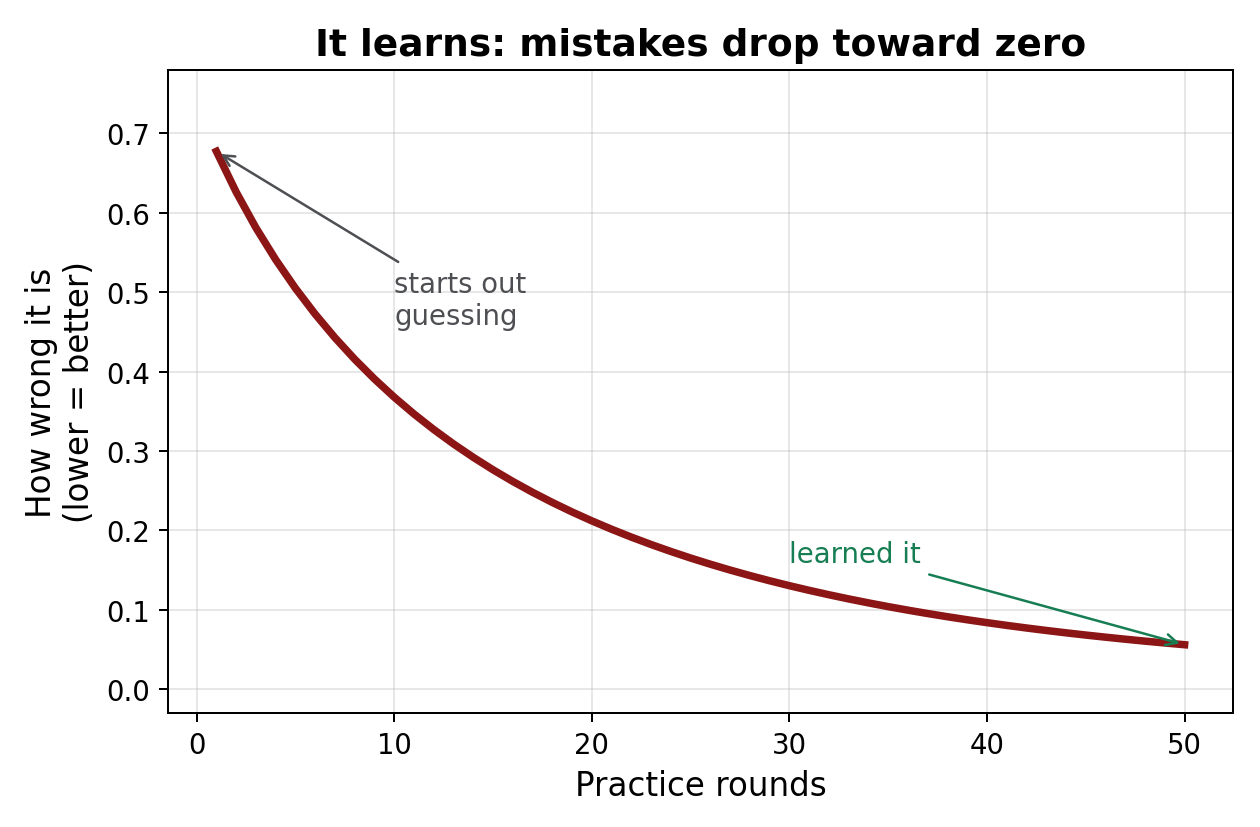
\includegraphics[width=0.86\linewidth]{assets/loss_curve.png}
      \end{column}
    \end{columns}
  \end{block}

  \begin{alertblock}{The update rule, explicitly}
    Run the circuit, get $P(\text{YES})$; the \textbf{miss} is $e=P(\text{YES})-\text{label}$.
    For each dial's angle $\theta$, get its \textbf{slope} by re-running the circuit with
    that angle shifted $\pm\tfrac{\pi}{2}$, then step the dial against the miss:
    \begin{align*}
      \text{slope} &= \tfrac12\!\left[\,P(\theta{+}\tfrac{\pi}{2}) - P(\theta{-}\tfrac{\pi}{2})\,\right]\\[2pt]
      \text{dial}  &\leftarrow \text{dial} - \eta\,(\,e \times \text{slope}\,)
    \end{align*}
    The shift-and-subtract is the \emph{parameter-shift rule} (how real quantum circuits
    get their gradients); $\eta$ is a small learning rate. Repeat over every sentence for
    $\sim$50 rounds.
  \end{alertblock}

\end{column}

\separatorcolumn
\end{columns}
\end{frame}

\end{document}
